\begin{figure}
    \centering
    \captionsetup[subfigure]{labelformat=empty}
\begin{subfigure}{.5\textwidth}
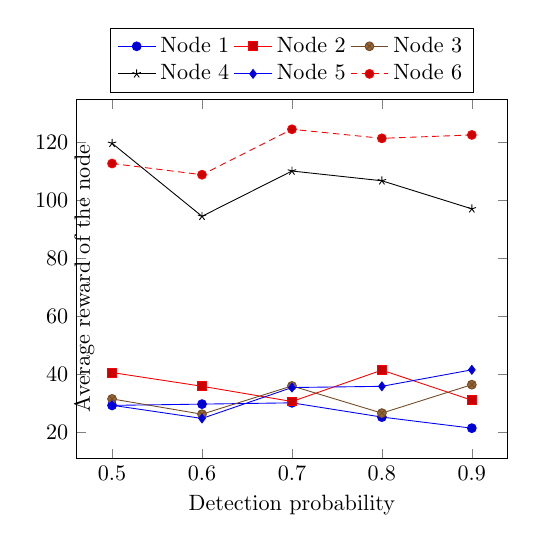
\begin{tikzpicture}[scale=0.8]
\begin{axis}[
  xlabel={Detection probability},
  ylabel={Average reward of the node },
  y label style={at={(0.06,0.5)}},
  xtick={0.5,0.6,0.7,0.8,0.9,1.0},
  legend style={at={(0.5,1.2)},cells={align=right}, anchor=north,legend columns=3},
  grid style=dashed,
]

\addplot+[]
    coordinates {
(0.5,29.2207587022)(0.6,29.6591500811)(0.7,30.107769581)(0.8,25.1808225374)(0.9,21.3501334315)
};

\addplot+[]
    coordinates {
(0.5,40.5649596864)(0.6,35.8317201966)(0.7,30.5615817425)(0.8,41.4017616625)(0.9,31.0018428294)
};

\addplot+[]
    coordinates {
(0.5,31.4601711216)(0.6,26.1715912622)(0.7,35.9427616495)(0.8,26.5488358659)(0.9,36.3780765072)
};

\addplot+[]
    coordinates {
(0.5,119.788927983)(0.6,94.566243579)(0.7,110.212449824)(0.8,106.844518821)(0.9,97.138069126)
};

\addplot+[]
    coordinates {
(0.5,29.2697135288)(0.6,24.7098561839)(0.7,35.3909999115)(0.8,35.8083893589)(0.9,41.5087141375)
};

\addplot+[]
    coordinates {
(0.5,112.808511307)(0.6,108.932780706)(0.7,124.631408718)(0.8,121.507931814)(0.9,122.678991306)
};

\legend{Node 1, Node 2, Node 3, Node 4, Node 5, Node 6}
\end{axis}
\end{tikzpicture}

\caption{Scenario a)}
\label{fig:nodeimp_single}
\end{subfigure}
\begin{subfigure}{.33\textwidth}
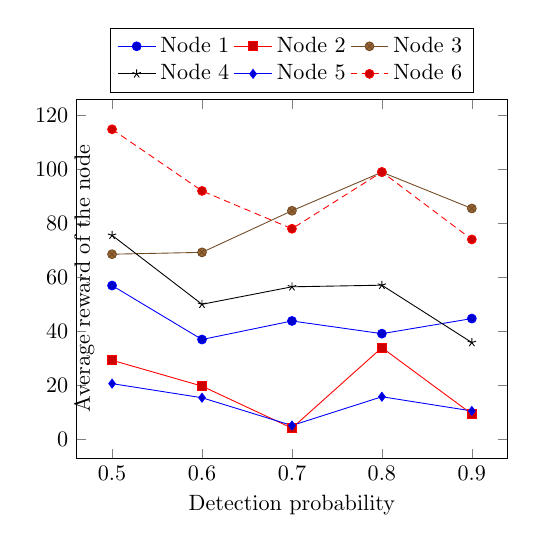
\begin{tikzpicture}[scale=0.8]
\begin{axis}[
  xlabel={Detection probability},
  ylabel={Average reward of the node },
  y label style={at={(0.06,0.5)}},
  xtick={0.5,0.6,0.7,0.8,0.9,1.0},
  legend style={at={(0.5,1.2)},cells={align=right}, anchor=north,legend columns=3},
  grid style=dashed,
]

\addplot+[]
    coordinates {
(0.5,57.0711574474)(0.6,37.0782125822)(0.7,43.9471043804)(0.8,39.2446371458)(0.9,44.8363801675)
};

\addplot+[]
    coordinates {
(0.5,29.4097815394)(0.6,19.8278112984)(0.7,4.26428571429)(0.8,34.0706693208)(0.9,9.49928571429)
};

\addplot+[]
    coordinates {
(0.5,68.6596096998)(0.6,69.339332514)(0.7,84.7438538657)(0.8,99.0264041517)(0.9,85.5894326243)
};

\addplot+[]
    coordinates {
(0.5,75.6609039908)(0.6,50.1243516403)(0.7,56.5923700845)(0.8,57.1874277411)(0.9,35.9649500717)
};

\addplot+[]
    coordinates {
(0.5,20.7573450249)(0.6,15.5267400966)(0.7,5.25375523139)(0.8,15.8992854434)(0.9,10.6415647894)
};

\addplot+[]
    coordinates {
(0.5,114.89762846)(0.6,92.0949728442)(0.7,78.0795310037)(0.8,99.102629324)(0.9,74.1266846482)
};

\legend{Node 1, Node 2, Node 3, Node 4, Node 5, Node 6}
\end{axis}
\end{tikzpicture}

\caption{Scenario b)}
\label{fig:nodeimp_topo1_multiple}
\end{subfigure}
    \caption{Results for single and multiple attackers - Scenarios a) and b)}
    \label{fig:mdp-result-topo1}
\end{figure}